\begin{quote}
	\textit{``The major challenge for the future will be effectively and cheaply to shift the sense of presence from one's own body to another, without replacing or excluding the physical world in which we all exist.''}
\end{quote}
\hfill \textit{Waterworth and Waterworth}~\cite{Waterworth2014}
\\
\\
%=========================================================================================================
%=========================================================================================================

\label{introduction}

%=========================================================================================================

A tourist steps into a 15th century chapel. Although the chapel is in remarkable condition for a building that is over 500 years old (it is even still in active use!) it looks markedly different today than it did when it was first built back in 1450. The tourist dons a head-mounted display, which via a pair of front mounted cameras allows her to still see where she is going as she starts to explore the chapel. Once in the centre of the building, she stops walking and presses a button on a controller that she holds in her hand. Her view of the chapel around her disappears and is replaced with an immersive virtual reconstruction of the chapel as it stood over 500 years ago. The view changes appropriately as she turns her head, allowing her to look all around at how the chapel used to be. She releases the button and is returned to the present day, where she continues walking through the chapel until she reaches the altar. She presses the button again and once more her view switches to that of the virtual chapel, which has moved to match her new position at the altar, allowing her to inspect its 1450 counterpart.

This is not an augmented reality system which superimposes virtual objects upon the real world. This is a \textit{parallel reality} system that allows her to switch between seeing the real world and the equivalent vantage in a complete, immersive virtual environment, allowing access to a level of tandem virtuality unprecedented of augmentations.

\afterpage{
\begin{figure}[h]
	\begin{center}
	   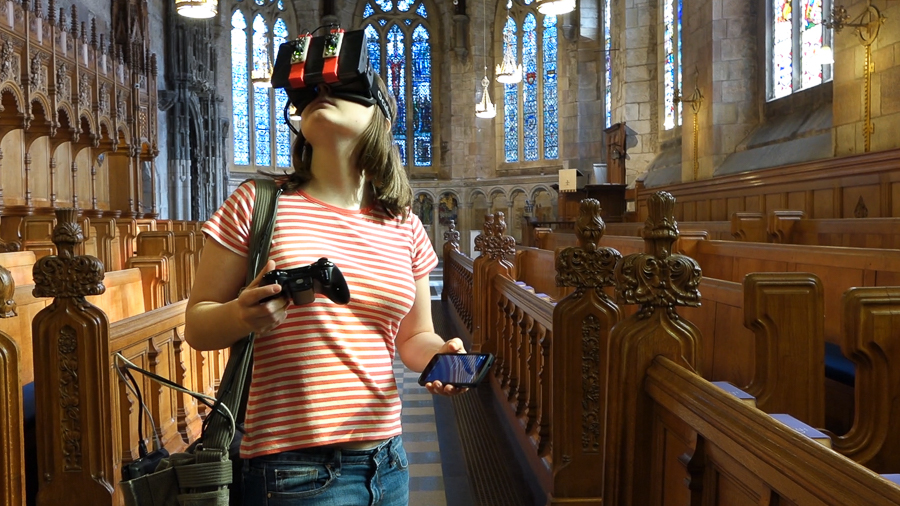
\includegraphics[width=\textwidth]{participant-f-2.jpg}
	\end{center}
	\label{participant-f-2.jpg}
	\caption{The \textit{Mirrorshades} parallel reality platform in use at a 15th century chapel\protect\footnotemark .}
\end{figure}

\footnotetext{ This image is taken from a video that is available to view online at \url{https://www.youtube.com/watch?v=UsDRPjDwr8A}}
}

%=========================================================================================================

\section{Parallel Reality}
\label{intro-parallel-reality}
The central theme of this thesis is the concept of `parallel reality', a new category of alternate reality defined thus;

\vspace{7mm}

\textbf{Parallel Reality:} A system comprising two environments, one real and the other virtual, each complete unto itself and wherein the user may freely switch between them.

\vspace{7mm}

%=====================

The concept of alternate realities has become a mainstay both of science fiction and of serious academic research, with the concept of other worlds and how we can either visit them or bring them into our real world keeping authors and scientists alike fascinated for decades. The concept of these `virtual worlds' dates back far into human history, long before mankind's invention of the transistor and the computers that would subsequently harness it.

\begin{quote}
	\textit{``Virtual worlds, or as we will now more broadly define them, immersive experiences delivered through the human imagination, have their origins in deep prehistory. Whether these varieties of nonphysical, dreamlike realities were communicated by our ancestors through the imitation of animals, the incarnation of spirits, the painting of scenes on the stone canvasses of caves, the holding of ceremonial rites in temples, or the elaboration of the human story through the fount of theater, humans have craved and crafted virtual-world experiences from the dawn of artistic and linguistic expression.''}~\cite{Damer2014}
\end{quote}

Within this thesis we are concerned with those alternate realities that through means of computers or other apparatus modify, mediate or create the environmental stimuli received by a subject's senses. While some alternate reality endeavours have explored the mediation of multiple human senses, from Morton Heilig's 1950's `Sensorama' experience that presented its occupant with a motorcyle ride through combination of film, sound, wind, vibration and odor~\cite{Rheingold1992}, to present day experiences that combine multiple computer generated sensory data such as the Birdly full body flight simulator\footnote{\url{http://birdly.zhdk.ch/}}, many are focussed upon visual stimuli alone, with other senses suspended or separated, bracketed into a \textit{``different stream of awareness''}~\cite{Adams2014}.

\begin{quote}
	\textit{``Sight plays such a prominent part in the mental life that the field of vision is sometimes considered almost synonymous with the field of attention.''}~\cite{Lucas1951}
\end{quote}

The 1990s saw a surge of interest around \textit{virtual reality}, promising to immerse users via a head mounted display (HMD) into 3D virtual environments. However with hardware and software simply not advanced enough to meet the news and media generated hype, the virtual reality bubble burst and was largely ignored as a consumer platform for gaming and media consumption.

The advent and mass adoption of the smartphone beginning in the early 2000s, with its combination of location sensing (GPS) and orientation sensing (accelerometer and gyroscope) capabilities in a portable package with a screen, camera and Internet access, led to a surge of \textit{augmented reality} applications, which overlaid virtual objects and data upon the view of the real world captured by the phone's rear-facing camera.

The early 2000s also saw the rise of a next generation of persistent multi-user virtual environments, self proclaimed `virtual worlds', with a focus on 3D3C (3D, Community, Creation and Commerce)~\cite{Sevan2008}, including Second Life\footnote{\url{http://secondlife.com/}} from Linden Lab and its open source implementation OpenSim\footnote{\url{http://opensimulator.org/}}. The scientific research potential of these virtual worlds~\cite{Bainbridge2007} led to numerous projects that explored their utility for subjects as diverse as education~\cite{Allison2012}, virtual heritage~\cite{Kennedy2013}, building automation systems\footnote{\url{http://www.ugotrade.com/2007/07/02/eolus-makes-leap-to-3d-internet-on-second-life/}}, data centre visualisation\footnote{\url{http://www-03.ibm.com/press/us/en/pressrelease/23565.wss}} and standards design~\cite{Gelissen2011a}, amongst others.

One such project, led by Joshua Lifton at MIT's Media Lab, introduced \textit{cross reality} as a new category of alternate reality in which the real world and a virtual environment (in this case provided by Second Life) are connected by sensor and actuator infrastructure, allowing bidirectional exchange of media and control information between the two environments, such that actions and events in one can manifest in the other~\cite{Lifton2007a}. This endeavour aimed to mitigate what Lifton identified as the \textit{vacancy problem}, which described how a person interacting with a virtual environment becomes unaware of their real environment and vice versa, by virtue of not having \textit{``the means to be in more than one place (reality) at a time''}.

The vacancy problem remains an important consideration as we move rapidly into a world where the ubiquity of technology, wireless communications and the explosive popularity of social networking services (SNS) heralds the coming of an era in which maintaining a virtual presence (whether 3D or on Facebook) while continuing to function in the real world becomes not just desirable, but the norm, creating instances of \textit{polysocial reality}~\cite{Applin2012} (see also the opening quote to this chapter) wherever we go.

It is here in the story of alternate realities that this thesis enters. Taking one of the core concepts of cross reality, that of tandem real and a virtual environments both complete unto themselves, and extending it to allow the user to engage \textit{visually} with both environments wherever within them they may be, gives rise to parallel reality. With the recent resurgence of interest in HMD based virtual reality, thanks largely to the introduction by Oculus\footnote{\url{https://www.oculus.com/}} of their Rift developer kits that leverage advances in display technology to overcome the shortfalls of the 90s virtual reality fad, and the introduction of novel smartphone based indoor positioning technology from IndoorAtlas\footnote{\url{https://www.indooratlas.com/}}, the \textit{Mirrorshades} parallel reality platform was developed and evaluated as a first foray into this exciting new take on our realities. Where cross reality permitted users an indirect insight into the other environment by means of sensors and actuators, parallel reality grants them the ability to switch between direct visual engagement with each environment - to at one moment view their real surroundings and at the next to view the equivalent vantage in the immersive parallel virtual environment.

%=========================================================================================================

\section{Contributions}
\label{intro-contributions}
The contributions of this thesis can be summarized as follows;

\begin{itemize}
	\item The introduction of parallel reality as a new category of alternate reality that allows users to experience complete real and virtual environments in tandem and represents an avenue for further mitigation of the vacancy problem.
	\item The framing of parallel reality through a thorough investigation and extension of previous taxonomies that classify and distinguish between alternate reality terminologies.
	\item The presentation of the combined Milgram/Waterworth model for visualising alternate reality experiences, including those of parallel reality systems.
	\item Development of a preliminary parallel reality platform, the Virtual Time Window, through extension of the Second Life client.
	\item Development of a second parallel reality platform, dubbed Mirrorshades, that combines new virtual reality hardware with novel indoor positioning technology.
	\item Evaluation of the Mirrorshades platform through user studies of a real world use case study within the realm of cultural heritage, including the discussion and application of an established presence questionnaire to a parallel reality experience.
	\item Creation and discussion of a set of best practices for future parallel reality endeavours.
\end{itemize}

%=========================================================================================================

\section{Document Overview}

Chapter \ref{chapter-background} surveys the ecosystem of alternate realities, including methods and taxonomies for classifying, categorising and distinguishing between different alternate reality terms, in order to frame the introduction of the parallel reality concept against existing techniques. Chapter \ref{chapter-vtw} describes the development of an initial tablet based parallel reality system, the Virtual Time Window, while chapter \ref{chapter-mirrorshades} details the development of the Mirrorshades HMD based parallel reality platform. Chapters \ref{chapter-eval-1} and \ref{chapter-eval-2} cover the investigation of the Mirrorshades platform through user studies at a cultural heritage site, the former comparing parallel reality against a more traditional scenario in which virtual reality has already come to be used at such sites and the latter investigating the benefits and drawbacks to different manners of parallel reality implementation, resulting in a set of best practice recommendations. Finally chapter \ref{chapter-conclusions} concludes the body of work and postulates on avenues for further investigation into the parallel reality concept.

%=========================================================================================================

%\section{Research Domains}

%\subsection{Virtual Reality}
%including imaging

%\subsection{Virtual Heritage}

%\subsection{Indoor Positioning}

%\subsection{Presence}

%=========================================================================================================

%From William Gibson's `The Gernsback Continuum' and beyond through contemporary cyberpunk literature

%``the reality games of Philip K Dick''~\cite{Sterling1988} and the almost constant virtual overlays of the real world described in Vernor Vinge's Rainbows End~\cite{Vinge2006}



%=====================
%On why alternate realities are predominantly visual?

%\textit{``visual ordination of intellectual knowledge''}

%\textit{``Seeing remains an insistent metaphor for all of cognition only because while the ocular lobes are merely one of our brain's tentacular connections to reality, they are among the most `conscious' of their capacity for information control.''}

%The Mediated Sensorium, Caroline A. Jones




%put into background chapter

%\textit{``virtual reality is a technology that convinces the participant that he or she is actually in another place by substituting the primary sensory input with data received produced by a computer''}~\cite{Heim1998}


%=====================


%can sound alone give us an alternate reality?
%Caroline A. James speaking on the work of Janet Cardiff and George Bures Miller
%\textit{``Cardiff brings segmentation into the present, crafting `sound walks' that layer an alternate reality over the fl\^aneur's perambulations - a fantastic elaboration of the kind of personal soundscape chosen by the iPod user.''}

%=========================================================================================================